\chapter{Vlastní řešení}  

V této části navrhneme podobu vlastního řešení problému specifikovaného v předchozích kapitolách. Návrh by měl nabízet jednoduché a vyhovující řešení vycházející ze stanovených požadavků a cílů. 

\section{Návrh}

Cílem práce je poskytnout konverzi \LaTeX\ souborů do PDF, čehož bude dosaženo pomocí webové služby. Tato služba bude poskytovat svoje rozhraní a funkcionalitu portálům Moodle a CourseWare. Jedná se o jednoduchou aplikaci s jediným účelem, tedy kompilace \LaTeX\ souborů do PDF. Tudíž není potřeba složité databáze, výsledný soubor PDF bude uložen do klasického souborového systému. 

\subsection{Platforma}
Na základě požadavků bude aplikace postavena na Java EE, což je platforma pro vývoj webových aplikací rozšiřující standardní Javu SE. Oproti ní poskytuje některé zásadní techniky navíc, jednu si tedy představme. 
\par
\textbf{Vkládání závislostí} (dependency injection) umožňuje objektu používat jiné objekty bez potřeby ho zatěžovat jejich vytvářením. Objekty, které můžeme takto vkládat, se nazývají beany a právě o jejich vytváření a zánik se stará Contexts and Dependency Injection (dále jen CDI) kontejner.
\\[12pt]
\par
Dále je potřeba specifikovat aplikační server. Ten poskytuje pro webové aplikace běhové prostředí, tedy zajišťuje správu databázových spojení apod. Na základě zkušeností je vybrán open-source Payara, který staví na GlassFish, o proti němu poskytuje častější aktualizace a opravy chyb. 

\subsection{Komunikace}
Pro komunikaci mezi klientem a serverem je vybráno REST Api. Poskytuje jednoduché rozhraní, se kterým je schopen komunikovat jakýkoliv systém pouze na základě znalosti struktury požadavků a odpovědí. Posílání zpráv bude postaveno nad protokolem HTTP pomocí GET a POST metod. Na obrázku \ref{fig:seq} je zobrazena komunikace mezi serverem a klientem. 

\begin{figure}[H]
	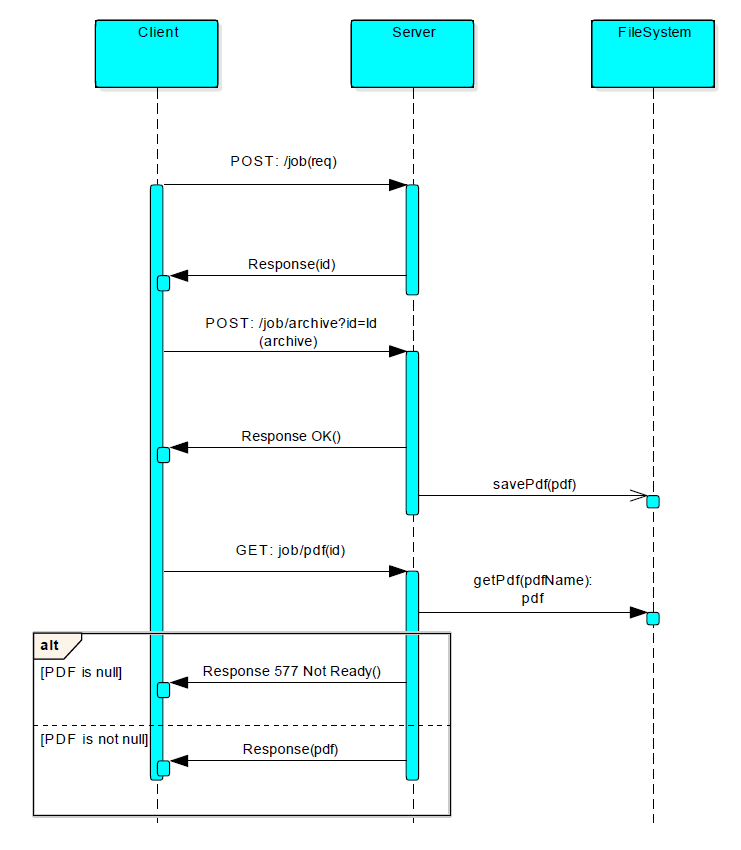
\includegraphics[width=0.9\textwidth]{diagram}
	\centering
	\caption{Sekvenční diagram}
	\label{fig:seq}
\end{figure}

Kompletní dokumentace k rozhraní se nachází na swagger\footnote{https://app.swaggerhub.com/apis/Tadky/Thesis/1}. Na ukázku vypíšeme alespoň používané zdroje:
\begin{itemize}
	\item \textbf{POST} {\ttfamily /job} - Slouží k předání požadavků na výsledné PDF.
	\item \textbf{POST} {\ttfamily /job/archive?id=<jobId>} - Musí obsahovat zip archiv s potřebnými soubory pro kompilaci.
	\item \textbf{GET} {\ttfamily /job/pdf?id=<jobId>} - Vrací výsledné PDF, pokud už je hotové.
\end{itemize}

\subsection{Zabezpečení}
Autentizace bude probíhat skrze tokeny, které budou mít dané portály přiřazené. Ty budou vygenerovány ručně a budou předány správcům portálů. Každá zpráva poslaná na server bude obsahovat token, který se bude ověřovat oproti tokenu uloženém v properties\footnote{Soubor v němž jsou data uspořádány klíč = hodnota} souboru.

\subsection{Kompilace}
Pro vytvoření PDF je nutné příslušně zkompilovat celý \LaTeX\ projekt. Pro úspěšnou kompilaci je potřeba, aby kompilátor měl k dispozici všechny balíčky, které jsou použity v projektu. Jsou tři způsoby, jak toho docílit.
\begin{enumerate}
	\item Stáhnout všechny balíčky již při instalaci kompilátoru
	\item Nainstalovat čistý kompilátor
		\begin{enumerate}
			\item Stáhnout několik balíčků a jenom ty se budou používat
			\item Získávat balíčky podle potřeby za běhu
		\end{enumerate}
\end{enumerate}
První možnost je zbytečná z důvodu mnoha nepoužívaných balíčků a velikosti na disku. Druhá možnost nabízí dvě podmožnosti, kde volba s přednastavenými balíčky vytváří omezení pro uživatele tudíž je může odrazovat od používání aplikace. Nejvíce vhodná se zdá poslední možnost, která eliminuje všechny neduhy předchozích, tím pádem je i zvolena.
\par
Na základě porovnání kompilátorů (sekce \ref{compilator}) z předchozí kapitoly je zvolen MikTeX, který poskytuje vše potřebné a nabízí vhodné funkcionality pro téma této práce např. doinstalovávání balíčku za běhu. Bude nainstalován ve verzi \enquote{Just enough TeX}, tudíž nebude obsahovat žádné balíčky. Ty se právě budou doinstalovávat až na požadavek při kompilaci.

\subsection{PDF úpravy}
Jelikož jsou kladeny požadavky na výsledný soubor PDF a bohužel kompilátory tyto úpravy nepodporují, je potřeba použít jiný nástroj, který bude umožňovat měnit soubor podle požadavků. Nejvíce vhodný se zdá PDFtk\footnote{https://www.pdflabs.com/tools/pdftk-server/}, který je pod GPL\footnote{Poskytuje svobodu šíření, provozování a upravování daného software.} licencí a nabízí vše potřebné. Tedy po zkompilování do PDF se za pomoci výše zmíněné aplikace aplikují požadavky, které byly obdrženy od klienta.

\subsection{Server}
V této fázi návrhu máme už všechny potřebné informace, aby mohl být zvolen operační systém a stanoveny požadavky na server. Jsou známy dvě omezující podmínky kladené na systém. První vychází z požadavků: operační systém musí být Debian nebo CentOS. Druhou určuje kompilátor. Jelikož byl zvolen MikTeX, který je podporován na Debian a Ubutnu, volba je jednoznačná. Na základě průniku je vybrán nejnovější Debian, tedy verze 9 s označením \enquote{stretch}. 
\par
Je také potřeba stanovit velikost diskového pole potřebného pro fungování. Jelikož nejvíce místa budou zabírat balíčky a potažmo výsledné pdf, budeme vycházet hlavně z těchto údajů. Přibližná velikost všech balíčků obsažených v plné verzi kompilátoru je zhruba 4GB, což bylo zjištěno na základě testovací instalace. Dále je potřeba odhadnout velikost všech PDF, které musí server uchovávat po dobu jednoho měsíce, v jeden moment. Horní odhad pro počet vytvořených PDF za den je 30 a pro velikost souboru je 10MB. Tedy na konci měsíce se může očekávat velikost cca 10GB. Tedy celkové požadované místo je 15GB.  
 



